\documentclass[12pt,letterpaper]{extarticle}

\usepackage{caption} % for the figure captions
\usepackage[osf]{mathpazo} % a nicer font
% this is a package for the citation formats: found this formulation sorted natbib errors when changing packages
%from http://tex.stackexchange.com/questions/54480/package-natbib-error-bibliography-not-compatible-with-author-year-citations
\usepackage[square,sort,comma,numbers]{natbib} 
\usepackage{amsmath} % package for equations
\usepackage{url} % package for urls
\usepackage{hyperref} % for hyperlinks
\usepackage[a4paper, total={6in, 9in}]{geometry}
\hypersetup{
     colorlinks   = true,
     citecolor    = gray
}
\usepackage{graphicx} % for the figures
\usepackage{pdfpages}
\hypersetup{linkcolor=blue}

\pagenumbering{gobble}

\graphicspath{ }


\begin{document}

%title

{\Huge\textbf{Where did we find our fishes?}\par}
\vspace{3mm}

\vspace{5mm}
The fossils on this table all come from a recent field trip our lab went on to Scotland. Scotland has a range of Devonian (420 to 360 million years ago) fossil sites - many of these come from a series of ancient lakes that lay over the northern part of Scotland.  The fishes lived on the edge of these lakes, but when they died they floated into the middle and sunk to the bottom, where they got buried and eventually fossilised. Some of the sites where we found fossils are marked on the map below. \newline

\begin{figure}[h!]
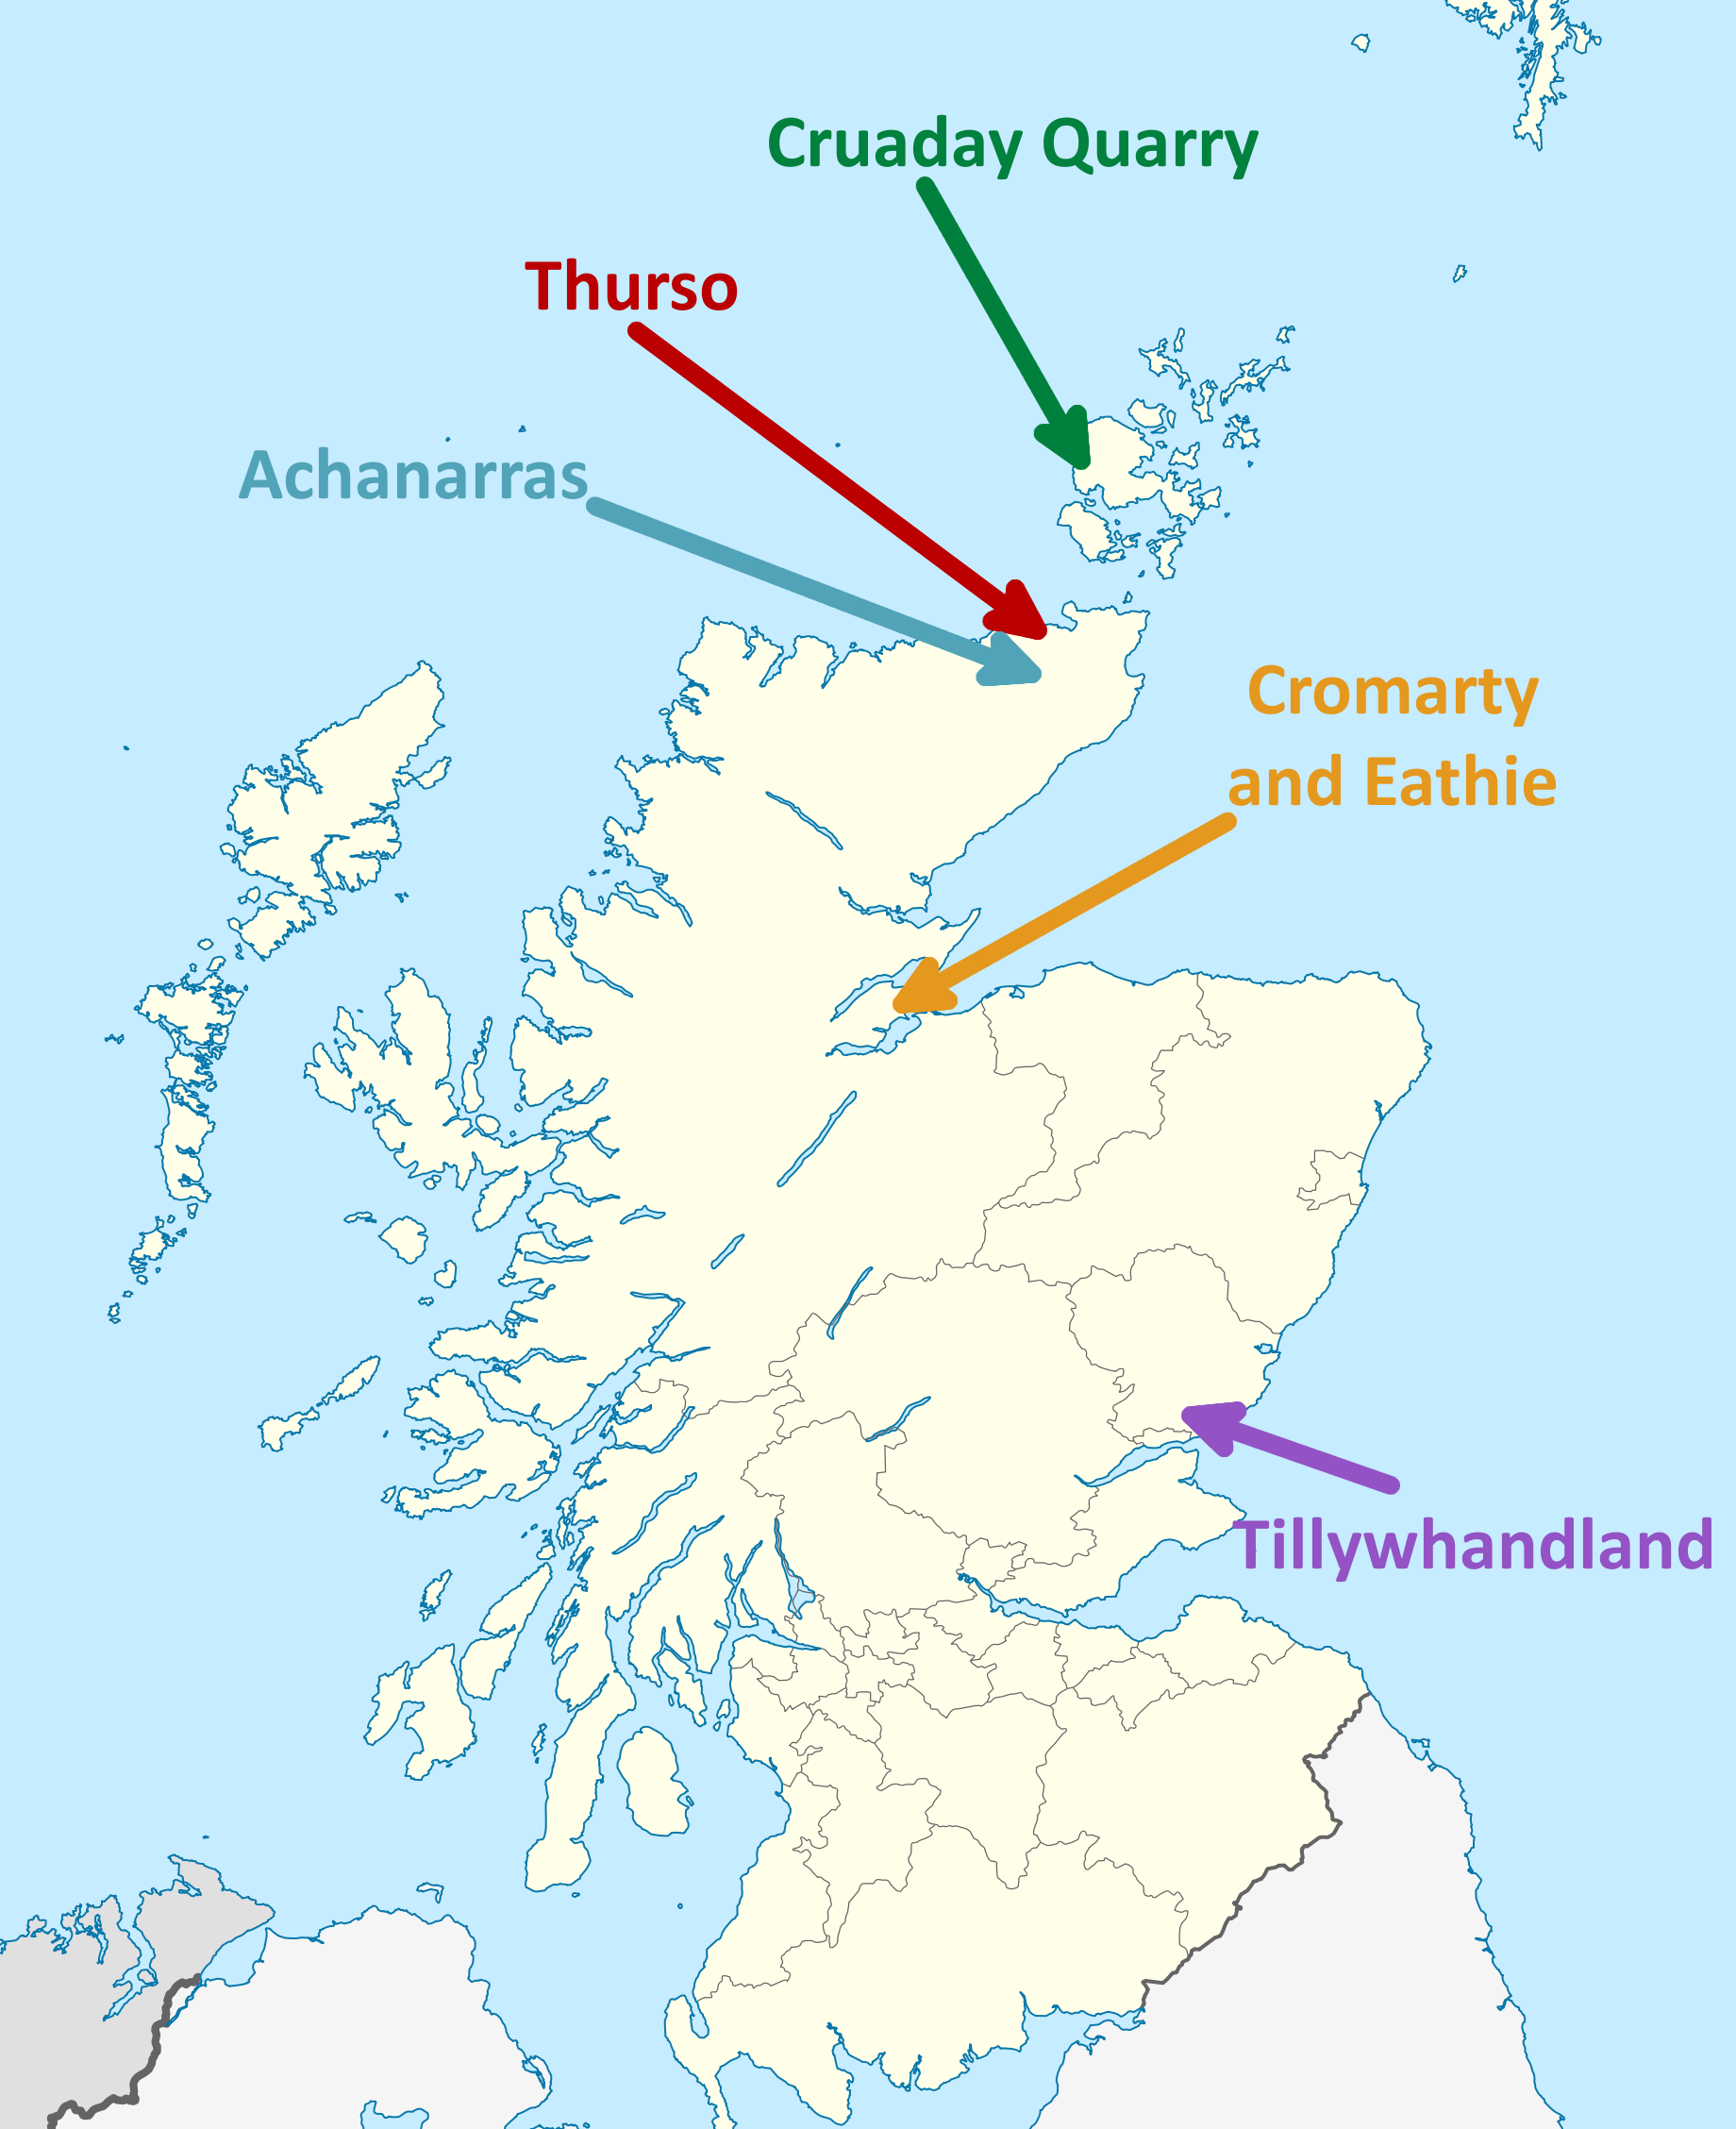
\includegraphics[scale=0.2]{Scotland_sites}
\centering
\end{figure}



\end{document}